
\section{Introduction}

Under consideration is a finite collection of mutually independent
real-valued random variables.  In one case, they are normally distributed
with possibly different means and variances.  In another case, they
are gamma distributed, with possibly different shapes and rates.  The parameters are considered known in either case, and of interest is 
the probability that a particular ranking of the variables occurs.  
It is routine to evaluate  this probability by Monte Carlo simulation; however
 a numerical solution is preferable in applications either  if the
probability itself is very small, or if very many instances of the
probability need to be computed.  This paper shows how the normal case
can be approximated by the gamma case and also how a version of the
Viterbi algorithm solves the gamma case.

Rank probabilities appear in various domains of statistics. 

\noindent
{\bf Preference ordering:} 
A toy example from Bayesian inference is illustrative.
A population of voters is sampled and each voter reports which of three 
candidates is his/her favorite for an upcoming election.  The
population is partitioned into three subsets, with unknown proportions 
$(p,q,r)$ of voters favoring each of the three candidates.
Similarly the sample is partitioned into three observed counts, $(a,b,c)$, say.
The likelihood $L(p,q,r)$ from simple random sampling is
$L(p,q,r) = p^a q^b r^c$. An analyst may be interested in preference
orderings, such as $E = ( p > q > r )$, or one of the five other versions,
as being relevant properties of the population under study.  The posterior 
probability of $E$ involves integrating a normalized version
 of  $L$ times a prior density over the event $E$.  Taking a flat prior,
for example, this posterior density is simply the density of
a Dirichlet distribution with shapes $(a+1,b+1,c+1)$.  It is well
known that the Dirichlet vector $(p,q,r)$ is equal in distribution
to a vector $(V_1/S, V_2/S, V_3/S)$, where $S=V_1+V_2+V_3$, and where
the $V_i$'s are independent gamma-distributed variables with common
rate and shapes $(a+1,b+1,c+1)$.  Thus to compute the posterior probability
of a preference ordering in the population, it is equivalent to compute
the probability that a sequence of independent gamma variates goes
in descending order.  For instance, if $n=30$ voters gave results
$(a,b,c)=(12,10,8)$, it turns out that the posterior 
 probability is $0.38$ that the population matches this empirical ordering.

**less toy from Tom Louis??**

\noindent
{\bf Seration:} 

\noindent
{\bf Other:} 


\noindent
{\bf Rank likelihood:} 
Consider a two-sample problem involving independent measurements
 from two source populations, with cumulative distribution functions
 $F$ and $G$.  Inferring differences between $F$ and $G$ is one of the 
 classical problems in statistics.  An interesting semiparametric method for
 this problem is based on rank likelihood (Pettitt, 1982; Doksum, 1987;
 Dabrowska, Doksum, and Miura, 1988; Cuzick, 1988; Tsukahara, 1997). 
  Ranks provide a natural and robust way to test the null 
 hypothesis that $F=G$ (e.g., Hoeffding, 1951; Kuk, 2009),
 but, in part for computational reasons,
 they have been less well developed beyond the null. 
 Rank-likelihood is the marginal probability of the ranks, expressed 
 as a function of parameters. It has been incredibly
 important for right-censored survival data (in the Cox proportional 
 hazards model), and may have further potential for other data structures.  

 Rank likelihood requires a semiparametric model for data.  Various 
 schemes are possible, but a compelling one is to assume that some
 unknown monotone transformation makes the data normally distributed
 with constant variance and with a population-specific mean.  The rank
 likelihood eliminates the unknown, nuisance transformation, and 
 involves a single parameter measuring the difference between 
  means on the transformed scale.
   To evaluate the rank likelihood is to evaluate the probability 
 that transformed data ({\em i.e.}, normal variates) achieve a particular
 ordering.  A rank likelihood for a similar gamma-based semiparametric
 model provides an approximation to the normal case (Section **). 

\noindent
{\bf Mixture-based clustering:}


\section{Gamma approximation to normal}

When its shape parameter is large, the gamma distribution is approximately
normal.  This property can be used to advantage to approximate
normal rank probabilities. 

Suppose we know real-valued means $\mu_1, \mu_2, \ldots, \mu_K$  and
positive variances $\sigma_1^2, \sigma_2^2, \ldots, \sigma_K^2$, 
and $Z_1, Z_2, \ldots, Z_K$ are mutually independent normal variables with
$Z_k \sim \, $Normal$(\mu_k, \sigma_k^2)$.  Of interest is the probability
of a given rank ordering.  Without loss of generality, consider
\begin{eqnarray}
\label{eq:norm1}
P\left( E_{\rm normal} \right) = P( Z_1 > Z_2 > \ldots > Z_K ).
\end{eqnarray}
Of course, $P\left( E_{\rm normal} \right) = 1/K! $ if all the means
are equal and all variances are equal.  
When $K=2$, the probability can be written as a tail probability for
one normal arising from the difference $Z_1-Z_2$, and so evaluation is also
elementary in this case.  In general, however, the probability 
depends in a complicated way on the means and variances. **citations**


A series of probabilities from gamma-distributed variables can be used
to approximate $P\left( E_{\rm normal} \right)$.  
 Recall that a gamma distribution 
with shape $\alpha >0$ and rate $\lambda >0$
has probability density proportional to 
$ v^{\alpha -1} \exp\{ -v \lambda \} $ for positive real $v$.
For each $n=1,2, \ldots$,
consider mutually independent variables $V_{n,1}, V_{n,2}, \ldots, V_{n,K}$
where $V_{n,k}$ is gamma distributed with shape parameter 
$\alpha_{n,k} = n/\sigma_k^2$ and rate parameter
$\lambda_{n,k} = \left( \frac{ n }{ \sigma_k^2}\right) \left\{  1 - \frac{\mu_k}{\sqrt{n}} + 
 	o\left( \frac{1}{\sqrt{n}} \right) \right\}.$
In comparison to (\ref{eq:norm1}), the gamma-rank probability is
\begin{eqnarray}
\label{eq:gam1}
P\left( E_{n, {\rm gamma}} \right) =
 P\left( V_{n,1} > V_{n,2} > \ldots  > V_{n,K} \right).
\end{eqnarray}

\begin{theorem}
With the shape and rate parameters as defined above,
\begin{eqnarray*}
\lim_{n\rightarrow \infty} P\left( E_{n, {\rm gamma}} \right) 
 = P\left( E_{\rm normal} \right).
\end{eqnarray*}
\end{theorem}
Thus a scheme to compute gamma-rank probabilities can be used 
to approximate the normal case.

In what follows we suppress the approximation level $n$ from the notation, 
and write things for
gamma variables $V_1, V_2, \ldots, V_K$ with shapes $\alpha_1, 
\alpha_2, \ldots, \alpha_K$ and rates $\lambda_1, \lambda_2, \ldots,
 \lambda_K$.
 When $K=2$, the probability~(\ref{eq:gam1}) 
 is equivalent to one for a single beta-distributed
 variable, and so the computation of
  $P\left(E_{\rm gamma}\right)$ is standard.  It seems that
 the general case has not received much attention.
  Newton and Chung (2009) report a formula
 for $P\left(E_{\rm gamma}\right)$ 
 in the case of integer-valued shape parameters:
\begin{eqnarray}
\label{eq:f1}
P\left(E_{\rm gamma} \right) = \sum_{m_1=0}^{\alpha_1 - 1} 
 \sum_{m_2=0}^{m_1+\alpha_2 -1 }
   \cdots \sum_{m_{K-1} = 0 }^{m_{K-2} + \alpha_{K-1} - 1 }
   p_1(m_1) \, p_2(m_2) \, \cdots \, p_{K-1}(m_{K-1}).
\end{eqnarray}
where the probability mass function $p_k(\cdot)$ is that of a
negative binomial random variable $M_k$ with shape $\alpha_{k+1}$ and
 scale $( \lambda_1 + \lambda_2 + \cdots + \lambda_k )/\lambda_{k+1}$,
which corresponds to the mass function:
\begin{eqnarray}
\label{eq:nb}
p_k(m) = \frac{ \Gamma( m+\alpha_{k+1} ) }{ \Gamma( \alpha_{k+1} )
  \, \Gamma(m+1) }
         \left( \frac{\lambda_{k+1}}{\Lambda_{k+1}} \right)^{\alpha_{k+1}} \,
         \left( \frac{\Lambda_k}{\Lambda_{k+1} } \right)^{m} 
\end{eqnarray}
for integers $m \geq 0$. Here $\Lambda_k = \sum_{j=1}^k \lambda_j$.
Representation~(\ref{eq:f1}) was found by embedding the gamma variables
in a certain collection of Poisson processes and then seeing the ordering
event as equivalent to an event on related count variables.  

It may happen that the first $K-1$ shape parameters $\alpha_k$ equal one,
in which case the sum in~(\ref{eq:f1}) collapses to a single term.
Beyond this special 
exponential case an explicit summation has to be evaluated.
Newton and Chung (2009) showed how the sum-product algorithm could be
used to redistribute elements of~(\ref{eq:f1}) in order to evaluate
$P(E)$ relatively efficiently (as in Kschischang {\em et al.} 2001) . 
The sum-product formulation speeds
up the naive summation, especially as $K$ increases, just as
the Baum-Welch forward-backward algorthm speeds up hidden-Markov
computatons.

When the summands in~(\ref{eq:f1})  are very small, there is
numerical instability in the evaluation of $P(E)$, even when
using the sum-product algorithm.  
Here we show how the Viterbi algorithm can be applied to 
identify the modal summand.  By factoring out the modal summand 
one gets an improved evaluation of $\log P(E)$. 
We also present an R package \verb+grankp+ for implementing the computation.

\section{The Viterbi connection}

Although there is no hidden Markov model (HMM) in the system of gamma
variables, the summation~(\ref{eq:f1}) is structurally equivalent to
that of a marginal probability for an HMM.  Obviously there are finitely
many terms in the sum, even though the negative binomial mass functions
are defined for all natural numbers, and it is convenient to define new
functions
\begin{eqnarray*}
h_1(m_1) & = & p_1( m_1 ) \, 1[ m_1 \leq \alpha_1 - 1 ]  \\ 
h_2(m_1,m_2) & = & p_2( m_2 ) \, 1[ m_2 \leq m_1 + \alpha_2 - 1 ]  \\
     & \vdots & \\
h_{K-1}(m_{K-2}, m_{K-1}) &= & p_{K-1}(m_{K-1}) \, 1[ m_{K-1} \leq m_{K-2} 
		+ \alpha_{K-1} -1 ].
\end{eqnarray*}
Since no index $m_k$ can exceed $A = \alpha_1 + \alpha_2 + \ldots + 
 \alpha_{K-1} - (K-1)$,
 it is reasonable to 
think of each of the $K-1$ sums in~(\ref{eq:f1}) as restricted to
$0, 1, \ldots, A$.  Re-writing~(\ref{eq:f1}),
\begin{eqnarray}
\label{eq:f2}
P(E) = \sum_{m_1 = 0}^A \sum_{m_2 = 0}^A \cdots \sum_{m_{K-1}=0}^A
  h_1(m_1) \prod_{k=2}^{K-1} h_k(m_{k-1}, m_{k} ) .
\end{eqnarray}
The linkages $h_k( m_{k-1}, m_k )$ between neighboring indices 
give the summation the same character as the summation required to
obtain a marginal probability in an HMM.

Recall the {\em log-sum-exp} formula for evaluating the logarithm
of a summation when
the summands are subject to numerical underflow (e.g., Press {\em et
 al.} 2007, page 844):
\begin{eqnarray*}
\log \left( \sum_i \exp(u_i) \right)   = \max_j (u_j) + \log\left( 
 \sum_i \exp[ u_i - \max_j (u_j) ] \right).
\end{eqnarray*}
To apply this formula in the present context, we must obtain the
vector $(\hat m_1, \hat m_2, \ldots, \hat m_{K-1})$ in the
integer lattice $[0,A]^{K-1}$
that maximizes the summand in~(\ref{eq:f2}).  We develop the Viterbi 
algorithm for this purpose as follows ({\em c.f.} Rabiner 1989).
For any $k \geq 2$ and $k \leq K-1$, we define the multi-variate function
\begin{eqnarray*}
T_k(m_1, m_2, \ldots, m_k ) = \log h_1(m_1)
 + \sum_{j=2}^{k} \log h_j( m_{j-1}, m_j ),
\end{eqnarray*}
where the $h_j$'s, from above, are truncated probability mass functions,
and allowing $\log(0) = -\infty $.  These are sub-components of
 the summands in~(\ref{eq:f2}), presented on the logarithmic scale.
Note that the final function
 $T_{K-1}(m_1, \ldots, m_{K-1})$ equals the log of the
entire summand, and so the optimizer of $T_{K-1}$ equals the
required mode $(\hat m_1, \hat m_2, \ldots, \hat m_{K-1})$.
From the multi-variate $T_k$'s we derive a sequence of univariate
functions (i.e., vectors) $\delta_2, \delta_3, \ldots, \delta_{K-1}$
as
\begin{eqnarray*}
 \delta_2(m) &=& \max_{m_1} \, T_2( m_1, m ) \\
 \delta_3(m) &=& \max_{m_1,m_2} T_3( m_1,m_2, m ) \\
  & \vdots & \\
 \delta_k(m) &=& \max_{m_1, m_2, \ldots, m_{k-1}} T_k( m_1, m_2, 
 \ldots , m_{k-1}, m ) \\
  & \vdots & 
\end{eqnarray*}
where, again, each $m$, $m_k$ takes values in $0, 1, \ldots, A$.
On the surface it seems that the computation of each $\delta_k(m)$
requires a search over $(A+1)^{k-1}$ values for $T_k$, but owing to
the pairwise linkages the computation can be done recursively much
more quickly than that. One fact driving the recursion is
that 
\begin{eqnarray*}
T_k( m_1, \ldots, m_k ) = T_{k-1}( m_1, \ldots, m_{k-1} )
   + \log h_k( m_{k-1}, m_k ).
\end{eqnarray*}
Additionally, maximization over multiple arguments can be done in
two steps, by maximizing in one set of arguments for each value of
the other, and then by maximizing this reduced profile in the other
arguments. Put together,
\begin{eqnarray*}
\delta_k(m) = \max_{m_{k-1}} \left\{ \max_{m_1, \ldots, m_{k-2} | m_{k-1} } 
 \left[  T_{k-1}(m_1, \ldots, m_{k-1}) + \log h_k(m_{k-1},m) \right] \right\}.
\end{eqnarray*}
The inner optimization is over $k-2$ variables and keeps $m_{k-1}$ fixed.
Thus the second term inside the optimization is constant, and can be 
moved out:
\begin{eqnarray*}
\delta_k(m) & = & 
  \max_{m_{k-1}} \left\{  \log h_k( m_{k-1} , m) +
  \max_{m_1, \ldots, m_{k-2} | m_{k-1} } 
   T_{k-1}(m_1, \ldots, m_{k-1})  \right\} \\
 & = & \max_{m_{k-1}} \left\{  \log h_k( m_{k-1} , m) +
       \delta_{k-1}( m_{k-1} )  \right\}. 
\end{eqnarray*}
This shows that the sequence of $\delta_k$ vectors can be computed recursively,
with a univariate optimization at each step.  During this recursion one
keeps track of arguments where the maxima occur, storing them in
vectors $\psi_k$, say:
\begin{eqnarray*}
\psi_k(m) = \arg\max_{ m_{k-1} } \left\{  \log h_k( m_{k-1} , m) +
       \delta_{k-1}( m_{k-1} )  \right\}. 
\end{eqnarray*}
Completing the Viterbi algorithm,
 backtracking is used to recover the mode:
\begin{eqnarray*}
\hat m_{K-1} &=&\arg\max_m \, \delta_{K-1} (m) \\
 \hat m_{k} &=& \psi_{k+1}( \hat m_{k+1} )\qquad
 {\mbox {\rm for $k = K-2, K-3, \ldots, 1$ }}.
\end{eqnarray*}

\section{Examples}

\subsection{Dirichlet ordering}
We illustrate the Viterbi computation using the Dirichlet ordering
problem from the Section~1.  Of interest is the posterior probability that
the population preference ordering for three candidates matches the
empirical ordering based on observed counts $(12,10,8)$. The counts
gives shapes $(\alpha_1,\alpha_2,\alpha_3)= (13,11,9)$ and 
the Dirichlet structure gives $\lambda_k=1$
for $k=1,2,3$.  Simplifying~(\ref{eq:f1}), the event probablity $P(E)$ is
\begin{eqnarray*}
P(E) = \sum_{m_1=0}^{12} \sum_{m_2 = 0}^{m_1+10} p_1(m_1) \, p_2(m_2)
\end{eqnarray*}
where, for $m \geq 0$,
\begin{eqnarray*}
p_1(m) &=& \frac{ \Gamma(m+11)}{\Gamma(m+1) \Gamma(11) }
  \left( \frac{1}{2} \right )^{ 11 } \, \left( \frac{1}{2} \right)^m  \\
p_2(m) &=& \frac{ \Gamma(m+9) }{ \Gamma(m+1) \Gamma(9) }
  \left( \frac{1}{3} \right )^{ 9 } \, \left( \frac{2}{3} \right)^m 
\end{eqnarray*} 
Reformatting the computation 
calls for both sums to range from $0$ to $A=22$
and requires objects
\begin{eqnarray*}
\log h_1( m_1 ) &= & \left\{ 
                  \begin{array}{ll}
			- \infty & {\mbox {\rm if $m_1 > 12$ } } \\
			\log p_1(m_1) & {\mbox {\rm else} } \\
		  \end{array}
		\right.
\end{eqnarray*}
and
\begin{eqnarray*}
\log h_2( m_1, m_2 ) &= & \left\{ 
                  \begin{array}{ll}
			- \infty & {\mbox {\rm if $m_2 > m_1+ 10$ } } \\
			\log p_2(m_2) & {\mbox {\rm else} } \\
		  \end{array}
		\right.
\end{eqnarray*}
Continuing, the bivariate $T_2(m_1,m_2)$ is the sum of these two functions,
and the vector $\delta_2$ has entries 
 $\delta_2(m) = \max_{m_1} T_2(m_1,m) $.  One finds that $\hat m_2=15$
is the argument maximizing $\delta_2(m)$, and then, backtracking, that
the argmax is $\hat m_1 =  9$ in the computation of $\delta_2(15)$. 
It happens in this case that $\hat m_1 = 9$ and $\hat m_2=15$ separately
maximize $p_1(m_1)$ and $p_2(m_2)$; in general the shape constraints 
can prohibit the joint mode from occurring at the conjunction of marginal
modes.

To utilize the {\em log-sum-exp} formula for computing $\log P(E)$, 
note
\begin{eqnarray*}
\log P(E) = \log p_1(\hat m_1) + \log p_2( \hat m_2 )
  + \log \left\{
     \sum_{m_1 = 0}^{12} \sum_{m_2=0}^{m_1+10}
     \frac{ p_1(m_1) \, p_2(m_2)  }{ p_1( \hat m_1 ) \, p_2 (\hat m_2 ) }
    \right\}
\end{eqnarray*}
**put in the numerical value for this example**

\subsection{Ordering genetic markers}

\subsection{Rank likelihood}
 

Consider a two-sample problem with independent measurements
 $X_1, X_2, \ldots, X_n$.  Let $\delta_1, \delta_2, \cdots, \delta_n$ 
 denote known binary indicators that distinguish the two source populations,
 and denote 
 the distribution of $X_i$ by $F$ when $\delta_i=0$ and by $G$ when 
 $\delta_i=1$.
 **start with Gamma ? **
 The semiparametric model driving the calculation is to express each observation
 in terms of a normal variable.  Let $Z_1, Z_2, \ldots, Z_n$
 be independent and identically distributed from a normal distribution with
 shape $a$ and rate $a$ (thus they have mean 1 and variance $1/a$).  (The
 approximate normality of this distribution, for large $a$, will be used
 to advantage in Section~4.)  
 Assume that for some continuous monotone increasing function $h()$, and
 for some $\lambda_a > 0 $,
 \begin{eqnarray}
\label{eq:model}
  X_i = h\left( \lambda_a^{ \delta_i } Z_i \right).
 \end{eqnarray}
The model is not so restrictive as it might seem, due to the absence
of any parametric assumptions on $h$.  Either $F$ or $G$ can take any
continuous distribution; the substantive restriction enters in the allowable
differences between the distributions.  To appreciate model~(\ref{eq:model}) 
further, consider $\theta = P( X_i < X_j )$ for $i$ in one group and $j$ in the other
(so $\delta_i=0$ and $\delta_j=1$).  Of course $\theta= 1/2$ when $F=G$; indeed
 $\theta$ is a parameter we can hope to infer from the ranks alone. We have
\begin{eqnarray}
\label{eq:theta}
 \theta &=& P(X_i < X_j) \\ \nonumber
        &=& P\left( h( Z_i ) < h( \lambda_a Z_j )    \right) \\ \nonumber
         &=& P\left( Z_i < \lambda_a Z_j \right) \\ \nonumber
         &=& P\left(  B < \lambda_a (1-B) \right) \\ \nonumber
         &=& P\left( B <  \frac{ \lambda_a }{ 1 + \lambda_a } \right) \\ \nonumber
\end{eqnarray}
where $B$ is a Beta-distributed variable with both shapes equal to $a$.
Thus  $\lambda_a$ and $\theta$ are directly related.

Information about $\theta$ is contained in the ordering of the observations, 
say 
\begin{eqnarray*}
E = \left\{ X_{\pi_1} < X_{\pi_2} < \cdots < X_{\pi_n} \right\}.
\end{eqnarray*}
The permutation $(\pi_1, \pi_2, \cdots, \pi_n)$ holds 
 the so-called {\em anti-ranks}
(they're the values returned by the \verb+R+ function \verb+order+.)
The rank likelihood for $\theta$ is
\begin{eqnarray}
\label{eq:rl}
 {\rm RL}(\theta) & = & P(E) \\ \nonumber
   & = & P\left(   X_{\pi_1} < X_{\pi_2} < \cdots < X_{\pi_n} \right) \\ \nonumber
   &=& P\left(  \lambda_a^{\delta_{\pi_1}} Z_{\pi_1} <
                \lambda_a^{\delta_{\pi_2}} Z_{\pi_2} <
                 \cdots
                < \lambda_a^{\delta_{\pi_n}} Z_{\pi_n}  \right)  \nonumber
\end{eqnarray}
owing to model~(\ref{eq:model}).  The $\lambda_a^{ \delta_{\pi_j} }$ factors
are constants in the calculation, and so ${\rm RL}(\theta)$ is expressible
 as the probability of an ordering of independent Gamma-distributed variables.
The algorithm from ** obtains.

Figure* demonstrates rank likelihood for 
the permeability example from Hollander and Wolfe (1999),
(example 4.1, page 110).
A nominal $95\%$ likelihood-based confidence interval for $\theta$
is $(0.08, 0.60)$ (dropping 2 log units from maximum), which differs
from other approaches. The interval by Halperin, Gilbert, and Lachin (1987)
 is $(0.13, 0.55)$ and by Sen (1967) is $(0.02, 0.58)$, as reported
in Hollander and Wolfe (1999) (page 131). (See also 
\verb+?wilcox.test+ in \verb+R+.) 

\begin{figure}
\centering
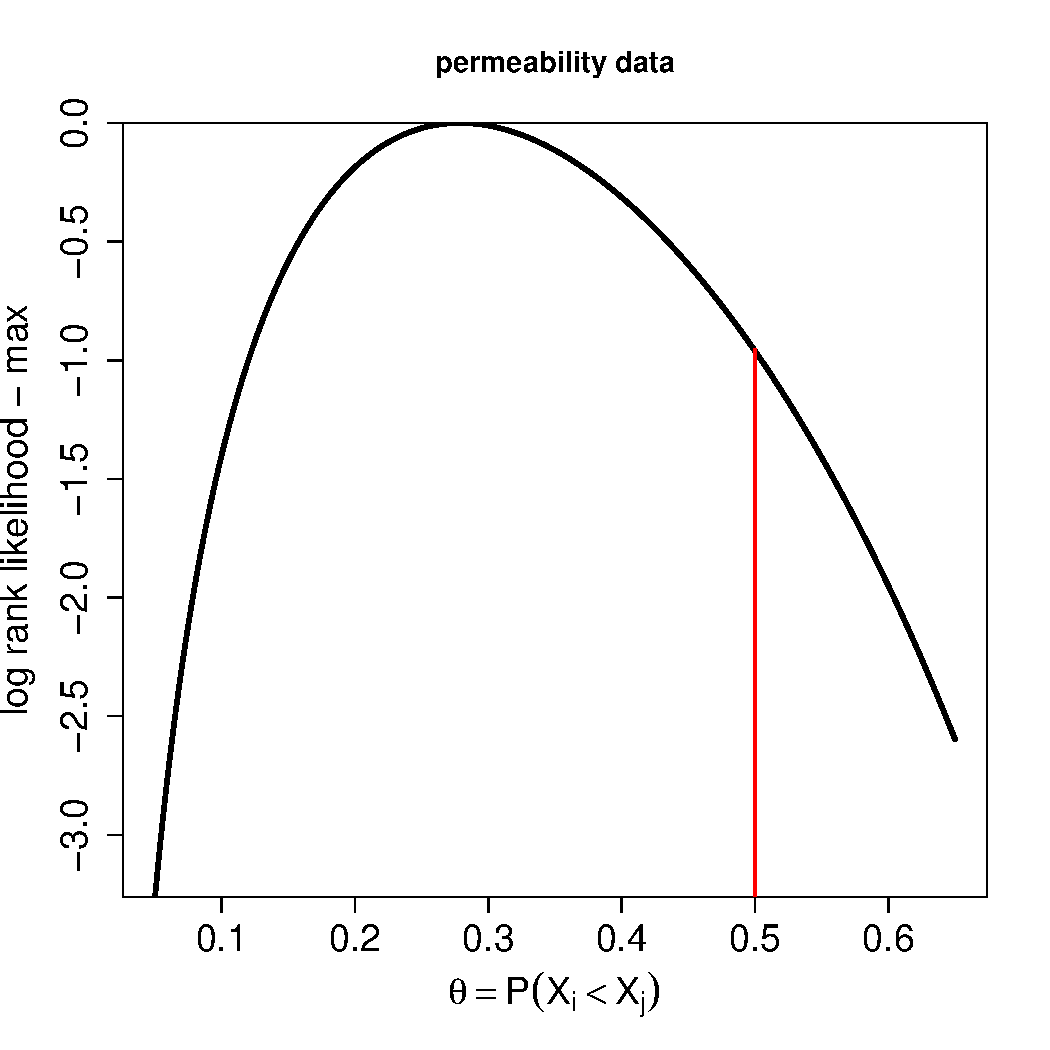
\includegraphics[height=.5\textheight]{R/figs/pd1.pdf}
\end{figure}

Numerical experiments showed that rank likelihood ${\rm RL}(\theta)$
is relatively insensitive to the shape parameter $a$ used in~(\ref{eq:rl}).
Since the Gamma distribution is approximately normal for large shapes,
(\ref{eq:f1}) may provide a useful numerical approach
to long intractable normal rank integral (citations).  The precise
connection to normality is presented in Section~4.  Roughly speaking,
model~(\ref{eq:model}) can be restated to say that some unknown
monotone transformation converts our data into  normally distributed scores.
Further, taking these scores to be standard normal in one sample $(\delta_i=0)$,
involves that in the other sample ($\delta_i=1$) 
 the scores are normal with mean $\sqrt{2} \Phi^{-1}(\theta)$   and unit
variance.  Here $\Phi$ is the standard normal cumulative distribution and
$\theta$ is as in~(\ref{eq:theta}).  (The phenomena is reminiscent of 
the bootstrap percentile method, which is justified when some unknown
monotone transform of the parameter estimator has a constant-variance
 normal distribution...citation....)

 **maybe equations and figure showing cdf $G$ when $F(x) = x$ on $(0,1)$. **




\section{Discussion}

 ... computation ...

...rank likelihood more generally

%% Hollander and Wolf, 1999, Nonparametric
%% Statistical Methods, 2nd edition, Wiley, example 4.1

\section*{Acknowledgements}... R version 2.10.1


\section*{Proof of theorem 1}

Each $V_{n,k}$ is approximately normal for large shape,
regardless of constraints on the rate parameters.

\noindent
{\bf Lemma:} 
 \textit{ Fix $k$, let $\alpha_{n,k} \rightarrow \infty$ 
 as $n \rightarrow \infty$, and take any positive rates $\lambda_{n,k}$. As $n \rightarrow \infty$,}
\begin{eqnarray*}
 W_{n,k} = \frac{ V_{n,k} - \alpha_{n,k}/\lambda_{n,k} }{
        \sqrt{ \alpha_{n,k}/\lambda_{n,k}^2 } }
   \longrightarrow_{d} {\mbox {\rm Normal}}(0,1) .
\end{eqnarray*}

\noindent
This can be confirmed by showing that the characteristic function
of $W_{n,k}$,
\begin{eqnarray*}
\phi_n(t) &= & E\left\{ \exp( i t W_{n,k} ) \right\} \\
 &=& \left[ \exp\left( -i t \sqrt{\alpha_{n,k}} \right) \right] 
     \left(  1 - it/\sqrt{
   \alpha_{n,k} }  \right)^{ -\alpha_{n,k} },
\end{eqnarray*}
converges to $\exp( - t^2/2 ) $.

To establish the theorem, 
 consider the event $E^n_{j,k} = [ V_{n,j} > V_{n,k} ]$
for distinct $j, k$ in $1, 2, \ldots, K$.  Clearly, $E^n_{j,k}$ is
equivalent to:
\begin{eqnarray}
\label{eq:balance}
W_{n,j} \sqrt{ \frac{ \alpha_{n,j} }{ \lambda_{n,j}^2 } }
+ \frac{ \alpha_{n,j} }{ \lambda_{n,j} } 
>
W_{n,k} \sqrt{ \frac{ \alpha_{n,k} }{ \lambda_{n,k}^2 } }
+ \frac{ \alpha_{n,k} }{ \lambda_{n,k} } .
\end{eqnarray}
The particular choices $\alpha_{n,k} = n/\sigma_k^2$ and
 $\lambda_{n,k} = \frac{n}{\sigma_k^2} \left\{ 1 - \frac{\mu_k}{\sqrt{n}}
 + o\left( \frac{1}{\sqrt{n}} \right) \right\}$ now come into play.
Multiply the both sides of (\ref{eq:balance}) by $\sqrt{n}$.  
While the $W$'s are stablizing at standard normals (by lemma), 
the multiplicative
factors are also converging. On the left,
\begin{eqnarray*}
\sqrt{n} \sqrt{ \frac{ \alpha_{n,j} }{\lambda_{n,j}^2 } }
 \longrightarrow \sigma_j
\end{eqnarray*}
as $n \rightarrow \infty$;
and similarly on the right side of (\ref{eq:balance}) 
 the factor multiplying $W_{n,k}$ converges to $\sigma_k$.
Some care is needed, since multiplication by $\sqrt{n}$ has also
inflated the additive terms on both sides of (\ref{eq:balance}). If we
further subtract $\sqrt{n}$ from both sides, the additive constant, on
the left, say, is
\begin{eqnarray*}
\sqrt{n} \left( \frac{ \alpha_{n,j} }{\lambda_{n,j} } \right) - \sqrt{n}
 &=&  \sqrt{n} \frac{n}{\sigma_j^2} \left[ \frac{n}{\sigma_j^2} 
  \left\{ 1 - \frac{\mu_j}{\sqrt{n}} + o\left( \frac{1}{\sqrt{n}} \right) 
 \right\}
  \right]^{-1} - \sqrt{n} \\
 &=&   \mu_j + o(1). 
\end{eqnarray*}
In other words, 
\begin{eqnarray*}
P( E^n_{j,k} ) = P\left\{ Z_{n,j} + o(1) > Z_{n,k} + o(1) \right\}
\end{eqnarray*}
 where $Z_{n,j} \longrightarrow_{d} \; $
 Normal$(\mu_j, \sigma_j^2 )$,
 $Z_{n,k} \longrightarrow_{d} \; $ Normal$(\mu_k, \sigma_k^2)$, and the 
$o(1)$ terms
represent deterministic sequences converging to zero, all as 
 $n \rightarrow \infty$.  Finally, put the pairwise events 
together, noting $E_{n,{\rm gamma}} = \bigcap_{k=2}^K E^n_{k-1,k}$,
to establish the result. $\Box$

\nocite{ksch,press,rab}



